\documentclass[9pt]{beamer}
\mode<presentation>
% input and font settings
\usepackage[utf8]{inputenc}		% for UTF8 input
\usepackage[T1]{fontenc}			% for T1 font family
\usepackage[english]{babel}		% for multilanguage input
% other settings
\usepackage{mathtools}
\usepackage{varwidth}
\usepackage{xcolor}
\usepackage{xfrac}
\usepackage{mathabx}
\usepackage[export]{adjustbox}
\usepackage{pgffor}
\usepackage{etoolbox}
\usepackage{xstring}
\usepackage{siunitx}
\usepackage{epstopdf}			% convert images to png
\epstopdfDeclareGraphicsRule{.tif}{png}{.png}{convert #1 \OutputFile}		% to covert TIF to PNG automatically
\AppendGraphicsExtensions{.tif}
%%% beamer settings
\beamertemplatenavigationsymbolsempty
%\usetheme{Boadilla}
\usetheme{Frankfurt}
\makeatletter
\@removefromreset{subsection}{section}
\makeatother
\setcounter{subsection}{1}



%%% author information
\author{Daniel \v{S}m\'{i}t}
\title{Crawling in the books}

\setbeamertemplate{itemize items}[default]
\setbeamertemplate{enumerate items}[default]

%%% document starts here
\begin{document}

%%% title frame
\begin{frame}{}
	\centering\Large
	\vspace{1em}
	{Crawling in the books\\}
	\vspace{1em}
	{Daniel \v{S}m\'{i}t\\}
	\vspace{1em}
\end{frame}

%%% the first section of slides
\section{Preparation}

\begin{frame}{Initial data manipulation}
	\begin{itemize}
		\item set up locale, clean missing and malformed data
		\item remove single ratings (user with 1 book, book with 1 rating)
		\item bundle ratings with age and geolocation of user
		\item filter LOTR books, or all Tolkien books (latter better for validation)
	\end{itemize}
\end{frame}

\begin{frame}{Insights}
	\begin{itemize}
		\item plot ratings by age, geolocation, user ratings
		\item compute rating-count, and mean rating for LOTR books
	\end{itemize}
	\begin{figure}
		\centering
		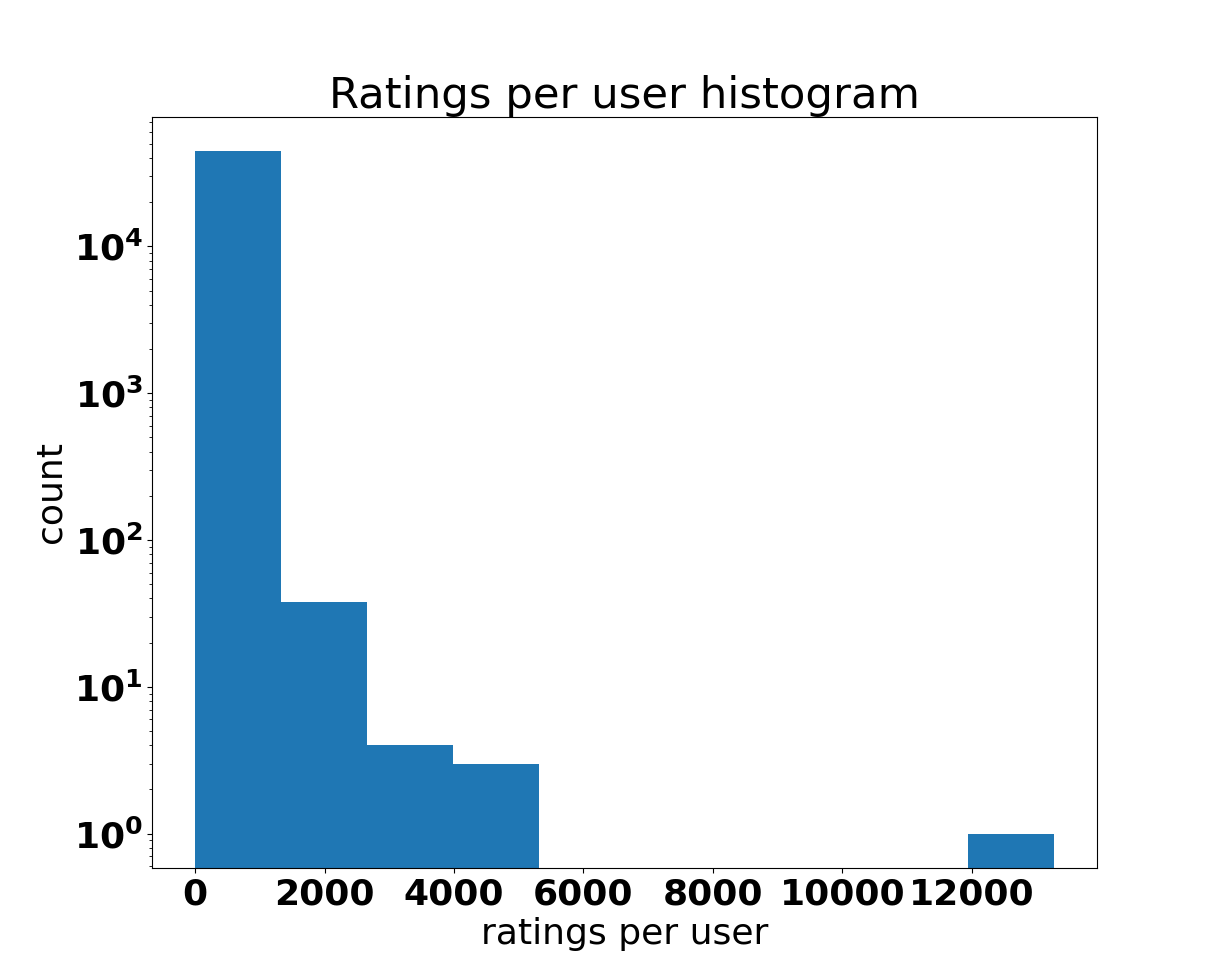
\includegraphics[width=0.7\textwidth]{../img/user-hist.png}
		\caption{User rating count histogram}
	\end{figure}
\end{frame}

%%% the second section
\section{Metrics}

\begin{frame}{General descriptors}
	\begin{itemize}
		\item general ratings statistics by book (count, mean rating, rating std)
		\item LOTR set books statistics (count, mean and std of rating)
		\item filtering by low count or low ratings
	\end{itemize}
\end{frame}

\begin{frame}{Rating group processing}
	Prepare user-based groups:\\
	\begin{itemize}
		\item select user-based rating groups $\{\gamma_i\}$ which contain at least one LOTR book
		\item \emph{count LOTR books} $\{\lambda_i\}$ and \emph{count all books} $\{\beta_i\}$ in each user group $i$ 
		%\item remove LOTR books from those groups 
	\end{itemize}
	Prepare metrics for each relevant books:\\
	\begin{enumerate}
		\item book belongs to $J>5$ rating groups $\{\gamma_1,\ldots,\gamma_J\}$ 
		\item mean number of LOTR books co-ocurring in rating groups $\Lambda =\frac{1}{J}\sum_{j=1}^{J} \lambda_j $
		\item mean size of rating groups $B = \frac{1}{J}\sum_{j=1}^J \beta_j$
		\item normalized weight as $W = \frac{\Lambda}{B}$
	\end{enumerate}
	Normalization gives high weight to groups where a book is accompanied by a large proportion of LOTR/Tolkien books.\\
	Note that we could have chosen another metric for normalized weight, possibly involving mean rating, or rating std.
\end{frame}

\begin{frame}{Ranking}
	Ranking of Tolkien co-rated books:\\
	\begin{itemize}
		\item compute weighted count $\kappa=W\cdot J$ of each book in $\{\gamma_1,\ldots,\gamma_J\}$
		\item rank book within Tolkien co-rated set by $\kappa$
		\item rank all general books by their count $\kappa'$ and filter Tolkien co-rated
		\item compute rank-gain for each book in Tolkien co-rated set $\kappa - \kappa'$ 
	\end{itemize}
	The rank gain represents how much more frequently a book co-occurs with Tolkien books relatively to other book as compared with its general Tolkien–-non-weighted occurence frequency.
\end{frame}

\begin{frame}{Relevance}
	Filter books with positive ranking gain $\kappa - \kappa' > 0$, and plot a scatter plot\\
	\begin{figure}
		\centering
		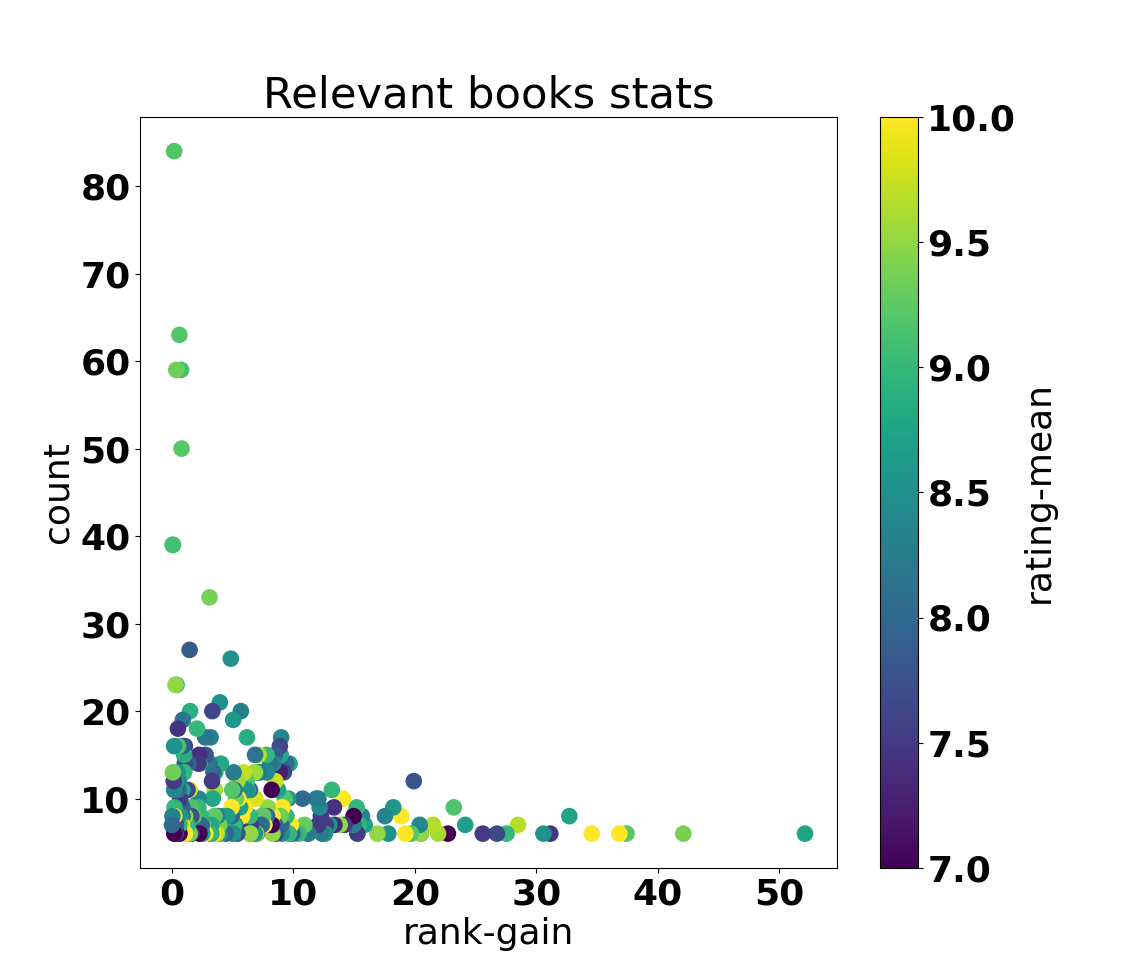
\includegraphics[width=0.6\textwidth]{../img/rank-scatter.png}
		\caption{Scatter plot of Tolkien co-rated book metrics}
	\end{figure}
	Note that we could select books for further analysis in different ways. Prefering those with highest rank gain, those with high count, or some sort of combined multi-objective (Pareto) selection.
\end{frame}

\section{Book groups}

\begin{frame}{Linking}
	Build a graph of links between books with positive ranking gain:\\
	\begin{itemize}
		\item create set of most common Tolkien books $\{\tau_k\}$ and rank gain books $\{\rho_l\}$, $\{\mu_m\}=\{\tau_k\}\cup\{\rho_l\}$
		\item count pair-wise co-ocurrence in the same rating group $\gamma_i$ for each pair $(\mu_m,\mu_n)$
	\end{itemize}
\end{frame}


\begin{frame}{Getting linked group}
	Estimate a group of books linked to LOTR books and to one another:\\
	\begin{itemize}
		\item create a normalized vector of weights $\tau^{(1)}$ as relative LOTR books count
		\item compute a vector of non-LOTR books linked ($\rho{-}\tau$ interactions) to this vector, $\rho^{(1)}$
		\item redistribute weights $\rho^{(n-1)} \rightarrow \rho^{(n)}$  by links between the books while weight std grows ($\rho{-}\rho$ interactions)
		\item select the top books from $\rho^{(n)}$
	\end{itemize}
	\\[1em]
	\begin{equation*}
		\begin{bmatrix}
			\rho^{(1)} \\
			{} \\
			0
		\end{bmatrix}
		=
		\begin{bmatrix}
			\rho{-}\rho \text{ interactions} & \vdots & \rho{-}\tau \text{ interactions} \\
			\hdotsfor{3} \\
			\tau{-}\rho \text{ interactions} & \vdots & \tau{-}\tau \text{ interactions}
		\end{bmatrix}
		\begin{bmatrix}
			0  \\
			{} \\
			\tau^{(1)}
		\end{bmatrix}
	\end{equation*}	
	\\[1em]
	\begin{equation*}
		\begin{bmatrix}
			\rho^{(n)}
		\end{bmatrix}
		=
		\begin{bmatrix}
			\rho{-}\rho \text{ interactions}
		\end{bmatrix}
		\begin{bmatrix}
			\rho^{(n-1)}
		\end{bmatrix}
	\end{equation*}
\end{frame}

\end{document}
